%\begin{document}

\chapter [Sensor Fusion and IMS]{Multisensor Data Fusion and Intersection Management Systems}

An intersection is a highly-dynamic scenario that can be monitored using a wide range of sensors. For this reason, an efficient and accurate fusion of the information is needed. This chapter is divided into two sections. In the first section a brief overview of multisensor data fusion is presented, remarking in different architectures proposed in the literature and different algorithms and frameworks used for this task. The second section contains a short review on intelligent transportation systems and intersection management systems, including a description of elements involved in the development of an IMS application. Finally, some projects that include multisensor data for intersection managing applications are presented.

\section{Multisensor Data Fusion}

Data fusion, also referred as mutisensor data fusion, information fusion or sensor fusion, has received several definitions from different authors in the literature. For example, Joint Directors of Laboratories defined data fusion as "multi-level, multifaceted process handling the automatic detection, association, correlation, estimation, and combination of data and information from several sources"\cite{White1991}. Luo refers to multisensor fusion and integration as "synergistic combination of sensory data from multiple sensors to provide more reliable and accurate information"\cite{Luo2002} and "to achieve inferences that are not feasible from each individual sensor operating separately"\cite{Luo2011}. Elmenreich states that sensor fusion is "the combining of sensory data or data derived from sensory data such that the resulting information is in some sense better than would be possible when these sources were used individually"\cite{Elmenreich2007}. In \cite{Bostrom2007} there is a compilation of more definitions of information fusion and the author summarize in his own statement as follows: "Information fusion is the study of efficient methods for automatically or semi-automatically transforming information from different sources and different points in time into a representation that provides effective support for human or automated decision making".  

% Elmenreich in [Elmenreich07]: Sensor fusion as "the combining of sensory data or data derived from sensory data such that the resulting information is in some sense better than would be possible when these sources were used individually"

%Khaleghi in [Kaleghi11]: "Multisensor data fusion is a technology to enable combining information from several sources in order to form a unified picture"

%White, JDL in [White91]: Data fusion as "multi- level, multifaceted process handling the automatic detection, association, correlation, estimation, and combination of data and information from several sources"

%Bostrom in [Bostrom07]: "Information fusion is the study of efficient methods for automatically or semi-automatically transforming information from different sources and different points in time into a representation that provides effective support for human or automated decision making"

%Luo refers to multisensor fusion and integration as "synergistic combination of sensory data from multiple sensors to provide more reliable and accurate information"\cite{Luo2002} and "to achieve inferences that are not feasible from each individual sensor operating separately"

All of previous definitions can be seen as a way to answer these three questions about data fusion:
\begin{itemize}
	\item {What is involved in data fusion?\\Combine, merge or integrate homogeneous or heterogeneous data.}
	\item {What is the aim of data fusion?\\Get a better representation of a process or the environment, infer underlying information, improve quality of the data.}
	\item {How to apply data fusion?\\Data fusion is a multi-level task, depending of the nature of the sensors, the final application and the environment.}
\end{itemize}

It is clear, now, that multisensor data fusion is a multidisciplinary field, because information in a typical process, flows from sensors to applications, passing through stages of filtering, data enhancement and data extraction. It is for this that knowledge in a wide range of fields are required, e.g. signal processing, machine learning, probability and statistics, etc. Also, it would be pointless to try to define a general method, technique or architecture that fits the requirements of any system, for applying data fusion in it.


%\subsection{Overview}
\subsection{Data Fusion Architectures and Models}

Although there is not a general rule of how to design or implement a sensor fusion system, many authors have proposed some models, architectures and guidelines for this task. Three well-known models are Waterfall model, JDL fusion model and Multisensor integration fusion model.

\subsubsection{Waterfall model}

Harris and Markin in \cite{Harris1998} and CITE, proposed a model named Waterfall, in which they describe the fusion process as an information flow through sensing to decision-making. They describe 3 levels of processing with 2 inner stages each ((\ref{WaterfallModel}). The first level is about transform the raw data from sensor to a better representation of the measured phenomena through signal processing and having in mind sensor models and nature of the process itself. The second level objective is to find a meaningful description of the data, reducing its volume while maximising information. This is done using feature extraction and pattern recognition techniques. The third level is the high level of the process in which situation assessment and decision making are performed, based on data available, configuration parameters, database information or human interaction. Finally, a feedback from high-level to low-level (sensor) is done, advising the whole system for re-calibration or reconfiguration.

\begin{figure}[ht!]
\centering
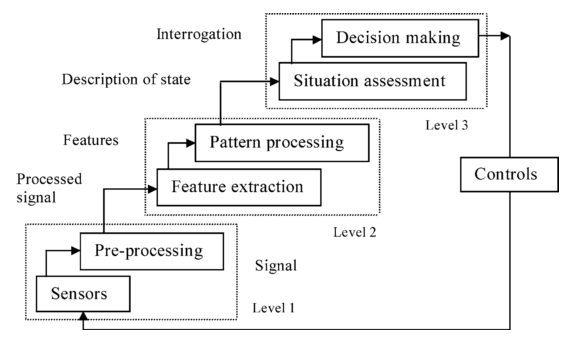
\includegraphics[scale=0.4]{fig/2/WaterfallModel.png}
\caption{Waterfall model (from \cite{Esteban2005}).}
\label{WaterfallModel}
\end{figure}

\subsubsection{JDL fusion model}

One of the first proposals of fusion architecture, and probably one of the most widely used, is the JDL fusion model, originated from the US Joint Directors of Laboratories and described by Hall and Llinas in \cite{Hall1997} and \cite{Llinas1998}. The JDL fusion model was conceived to aid the developments of military applications and comprises 5 levels of data processing at which data fusion could be done. These levels and a database are connected by a bus (\ref{JDLmodel}), and are not meant to be execute sequentially and can also be executed concurrently. 

\begin{figure}[ht!]
\centering
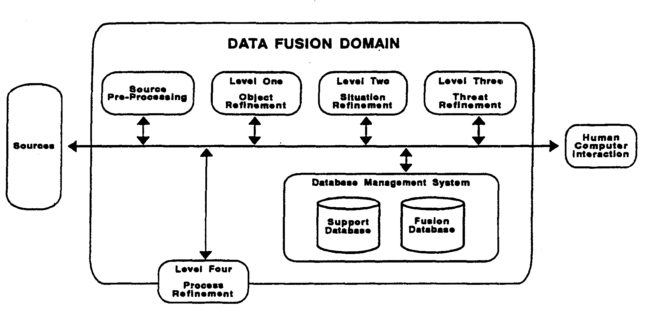
\includegraphics[scale=0.4]{fig/2/jdlmodel.png}
\caption{JDL fusion model. (from \cite{Hall1997}).}
\label{JDLmodel}
\end{figure}

The first stage, referred as level-0 is the source preprocessing in which raw data is handled to concentrate the more pertinent data for the current situation. The level-1 is for object refinement, starting with the alignment of the data in a commonly space-time reference frame. Then, performs identification and tracking of objects using different techniques. Situation refinement is at level-2, which takes observed and partially-observed object from level-1 and tries to find a contextual description between them. Level-3, threat refinement, is the level in which results from level-2 are interpreted looking for possible advantages and disadvantages for the system to operate, based on previous knowledge and predictions about executing an action.

\subsubsection{Multisensor Fusion Integration model}

Luo and Kai, in \cite{Luo1989, Luo1990}, proposed a full integration model for data fusion in which they define a three-level hierarchy for sensor fusion: data-fusion, feature-fusion and decision-fusion. This model separate MFI in five classes, based on Input/Output pair: Data in-data out fusion, data in-feature out fusion, feature in-feature out fusion, feature in-decision out fusion, and decision in-decision out fusion \cite{Luo2011} (figure \ref{fusionClasses}).

\begin{figure}[ht!]
\centering
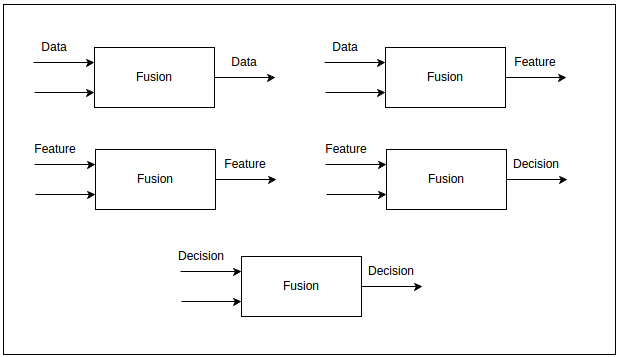
\includegraphics[scale=0.25]{fig/2/fusionClasses.png}
\caption{Five classes of Multisensor Fusion.}
\label{fusionClasses}
\end{figure}

Also, they made a clear distinction between multisensor fusion and multisensor integration, being the former the process in which information provided by a set of sensors is combined in any of the three levels aforementioned, and the latter is how sensor fusion could be integrated in a full system in order to assist in a particular task. As is depicted in figure \ref{MFIArch}, sensor fusion is an element of the whole MFI architecture, which also includes block for sensor managing tasks, like control, selection and registration of sensors, previously to the fusion process. A sensor processing stage and a system controlling module are also included after the sensor fusion stage.

\begin{figure}[ht!]
\centering
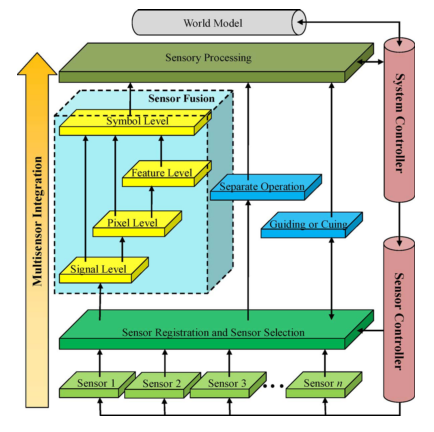
\includegraphics[scale=0.4]{fig/2/MFIArch.png}
\caption{Multisensor Fusion Integration architecture (from \cite{Luo2011}).}
\label{MFIArch}
\end{figure}

\subsection{Classification of Data Fusion Architectures}

Elmenreich in \cite{Elmenreich2007} classify fusion models in three categories: Abstract models, generic architectures and rigid architectures. Abstract model are not intended to show how to implement a sensor fusion system, but to explain which processes are done in it. Generic architectures gives an outline on how a system could be implemented in an application, but do not specify what type of hardware, database or communication system could be used. Finally, rigid architectures, are a good guide for implementation  of data fusion in certain applications, at the cost that several design decisions have been already taken, making expensive the migration to another architecture. 

In addition to models previously mentioned, there exists more proposal for data fusion architectures in literature, as can be viewed in table \ref{fusionModelsClas}.

% TODO: Change for a table
%\begin{figure}[ht!]
%\centering
%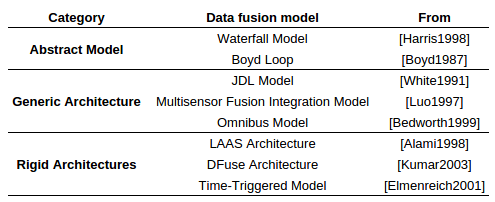
\includegraphics[scale=0.6]{fig/2/fusionModelsClas.png}
%\caption{Classification of some data fusion models}
%\label{fusionModelsClas}
%\end{figure}


\begin{table}
\footnotesize
\centering
\begin{tabular}{|c | c|}
\hline
\textbf{Category} & \textbf{Data Fusion Model} \\
\hline
\multirow{2}{*}{Abstract Model} & Waterfall Model \cite{Harris1998} \\
& Boyd Loop \cite{Boyd1987} \\
\hline
\multirow{3}{*}{Generic Architecture} & JDL Model \cite{White1991} \\
& Multisensor Fusion Integration Model \cite{Luo1989} \\
& Omnibus model \cite{Bedworth2000} \\
\hline
\multirow{3}{*}{Rigid Architecture} & LAAS Architecture \cite{Alami1998} \\
& DFuse Architecture \cite{Kumar2003} \\
& Time-triggered Model \cite{Elmenreich2001} \\
\hline
\end{tabular}
\caption{Classification of data fusion models}
\label{fusionModelsClas}
\end{table}


\subsection{Algorithms in Data Fusion}

Different types of algorithms have been used in implementing data fusion systems, depending on a variety of conditions like, level of fusion, type of the data, nature of environment, etc. Constrains like processing and memory limitations, centralised or distributed schemes, human-interactive or completely autonomous process, also determine which algorithms should be used in fusion process.

Luo in \cite{Luo2011} propose a classification for fusion algorithms based on the level of fusion. Low-level fusion refers to the merge of raw data or signals, mid-level fusion refers to the fusion of features and High-level fusion refers to the process of fuse decisions. Khaleghi in \cite{Khaleghi2013} describes a classification for fusion algorithms based on challenging problems that arise from the data to be fused, due to the variety of sensors and the nature of the application environment. This classification is not on the algorithms directly, but on the theory or framework in which they originate. Four types of data are enumerated: Imperfect data, correlated data, inconsistent data and disparate data. These two approaches of fusion algorithms classification are summarized in tables \ref{fusionAlgClasLuo} and \ref{fusionAlgClasKhaleghi}.

\begin{table}[ht!]
\footnotesize
\centering
\begin{tabular}{|c|c|c|c|}
\hline
\multicolumn{2}{|c|}{\textbf{Low level fusion}} & \textbf{Medium level fusion} & \textbf{High level fusion} \\
\hline
\multicolumn{2}{|c|}{\textit{Estimation methods}} & \textit{Classification methods} & \textit{Inference methods} \\
\hline
\parbox{2.5cm}{
	Recursive:
	\begin{itemize}[leftmargin=.07in]
		\item Kalman filter
		\item Extended Kalman filter
	\end{itemize}
	Non-Recursive:
	\begin{itemize}[leftmargin=.07in]
		\item Weighted average
		\item Least squares
	\end{itemize}
	}
 & 
 \parbox{2.5cm}{	 
 	Covariance-based:
	\begin{itemize}[leftmargin=.07in]
		\item Cross covariance
		\item Covariance intersection
		\item Covariance union
	\end{itemize}
	}
&
 \parbox{3cm}{	 
	\begin{itemize}[leftmargin=.07in, noitemsep]
		\item Parametric templates
		\item Cluster analysis
		\item K-means clustering
		\item Learning vector quantization
		\item Kohonen feature map
		\item Artificial neural networks
		\item Support vector machines
	\end{itemize}
	}
&
\parbox{3cm}{	 
	\begin{itemize}[leftmargin=.07in, noitemsep]
		\item Bayesian inference
		\item Particle filters
		\item Dempster-Shafer theory
		\item Expert systems
		\item Fuzzy logic
	\end{itemize}
	} \\
\hline
\end{tabular}
\caption{Classification of fusion algorithms based on level of fusion}
\label{fusionAlgClasLuo}
\end{table}

\begin{table}[ht!]
\footnotesize
\centering
\begin{tabular}{|c|c|}
\hline
\textbf{Data Problem} & \textbf{Framework} \\
\hline
\multirow{7}{*}{Imperfection} & Probabilistic \\
& Evidential \\
& Fuzzy reasoning \\
& Possibilistic \\
& Rough set theoretic \\
& Hybridization \\
& Random set theoretic \\
\hline
\multirow{2}{*}{Correlation} & Correlation elimination \\
& Correlation presence \\
\hline
\multirow{6}{*}{Inconsistency} & Sensor validation \\
& Stochastic sensor modeling\\
& Prediction \\
& Augmented state framework \\
& Combination rules \\
& Dempsters' rule \\
\hline
\multirow{3}{*}{Disparateness} & Dempster-Shafer theoretic framework \\
& Human-centered data fusion \\
& Hard-soft data fusion \\
\hline
\end{tabular}
\caption{Classification of fusion algorithms based on challeging problems in data}
\label{fusionAlgClasKhaleghi}
\end{table}

%\subsection{Laser and Video Data Fusion}

\section{Intersection Management Systems}

Intelligent Transportation Systems includes a wide range of applications and services transversal to many knowledge areas. For classifying those services, some taxonomies have been proposed like the ones presented in \cite[Ch.1]{Sussman2005} and \cite{Williams2008}. From described categories and classes, Advanced Traffic Management Systems have to be considered when an intelligent handling of traffic needs to be deployed.

One of the most desirable scenarios to improve efficiency and safety is an intersection. This because intersections are places where vehicles arrive from different directions at different velocities, increasing the chances for incidents and crashes. Choi \cite{Choi2010} states that 40\% of reported traffic accidents in the US, were intersection related. Also, in  \cite{CorporacionFondodePrevencionVial2010}, is reported that for Colombia in 2011, most of the accidents in the main cities were at intersections.

%El concepto de sistemas inteligentes de transporte (ITS), presenta un amplio campo de acci\'{o}n transversal a diferentes \'{a}reas del conocimiento e igualmente presenta una gran variedad de aplicaciones y servicios. Para la clasificación de estos servicios se han definido diferentes taxonom\'{i}as como las descritas en \cite[Ch.1]{Sussman2005} y en \cite{Williams2008}. De las clases y categor\'{i}as descritas, se tiene un subgrupo de los ITS que debe ser contemplado para cumplir con el objetivo de este proyecto, que es el que incluye los servicios y sistemas para la administraci\'{o}n y operaci\'{o}n del tr\'{a}fico (o Sistemas Avanzados de Administraci\'{o}n de Tr\'{a}fico, del ingl\'{e}s ATMS, Advanced Traffic Management Systems).
%
%Uno de los escenarios donde se busca mejorar la eficiencia y la seguridad usando estos sistemas son las intersecciones viales, ya que son puntos donde se encuentran veh\'{i}culos en diferentes direcciones a diferentes velocidades, lo cual incrementa la probabilidad de incidentes y choques. Cerca del 40\% de los accidentes de tr\'{a}nsito reportados en Estados Unidos en 2008, estaban relacionados con intersecciones \cite{Choi2010}. En Colombia, para el 2011 la mayor\'{i}a de accidentes en las principales ciudades del pa\'{i}s se concentraba en intersecciones \cite{CorporacionFondodePrevencionVial2010}.

%\section[Types of IMS]{Types of Intersection Management Systems}

Different types of applications and systems are conceived to address these issues. Some tasks performed by those are intersection monitoring, vehicles detection, incident warning, collision avoidance, among others. A typical Intersection Management System is composed by three main components: Data source, that could be infrastructure sensors, like inductive loops, range sensors or cameras, along vehicle sensors and traveling data; decision system, which is the core of the whole system, is in charge of analyse and process information provided by infrastructure, vehicles and authorities in order identify objects, recognise patterns, predict future incidents, control traffic and generate safe decisions and warnings alerts; and finally, is the presentation and displaying of the output of decision system, through infrastructure using dynamic signals, semaphore controlling, or using direct communication with drivers or vehicles through on-board visualisation/notification system. A block diagram of a generic IMS is presented in figure \ref{arch}

%Para afrontar esta problem\'{a}tica aparecen diferentes tipos de aplicaciones y sistemas para realizar tareas como monitoreo y administraci\'{o}n de intersecciones, detecci\'{o}n de veh\'{i}culos, advertencia de incidentes, prevenci\'{o}n de colisiones, entre otros. El esquema de comuniciaci\'{o}n de estos sistemas se basa en la interacci\'{o}n entre los veh\'{i}culos y la infraestructura, com\'{u}nmente dividida en 3 tipos: Comunicaci\'{o}n veh\'{i}culo a veh\'{i}culo (V2V), veh\'{i}culo a infraestructura (V2I) y la combinaci\'{o}n de las dos anteriores (V2X).

\begin{figure}[ht!]
\centering
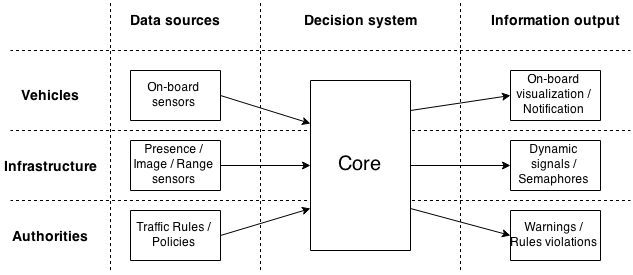
\includegraphics[scale=0.55]{fig/2/genericIMS.png}
\caption{Generic block diagram of an Intersection Management System.}
\label{arch}
\end{figure}



%En la figura \ref{arch}, se presenta un diagrama de bloques general de un sistema de administraci\'{o}n de una intersecci\'{o}n en donde se destacan 3 componentes: (a) Las fuentes de los datos, que pueden ser sensores en la infraestructura, como sensores inductivos, sensores de rango, c\'{a}maras, o sensores en el veh\'{i}culo. (b) Sistema  de decisi\'{o}n o administraci\'{o}n, que es el encargado de analizar la informaci\'{o}n de los veh\'{i}culos y el entorno, predecir incidentes futuros y enviar se\~{n}ales de alerta. y (c) La presentaci\'{o}n de informaci\'{o}n de control, que puede ser en la infraestructura con se\~{n}ales din\'{a}micas, control de los sem\'{a}foros, como tambi\'{e}n puede ser en el veh\'{i}culo mediante un dispositivo de visualizaci\'{o}n.

\subsection{Components in IMS application}

Intersection monitoring is a required task to be done within intelligent transportation systems for high-level applications like traffic analysis, counting and classification of vehicles or pedestrians, event prediction, incident detection and security and surveillance systems. Those applications have to take into account some of the elements depicted in figure \ref{arch}, so developments in IMS have a wide range of approaches and objectives. In order to study IMS applications, five components have been defined in which applications have their main focus, although mutiple components could be involved in the same development. In figure  \ref{imsComps} a graph is presented, showing aforementioned components and elements within them.

\begin{figure}[ht!]
\centering
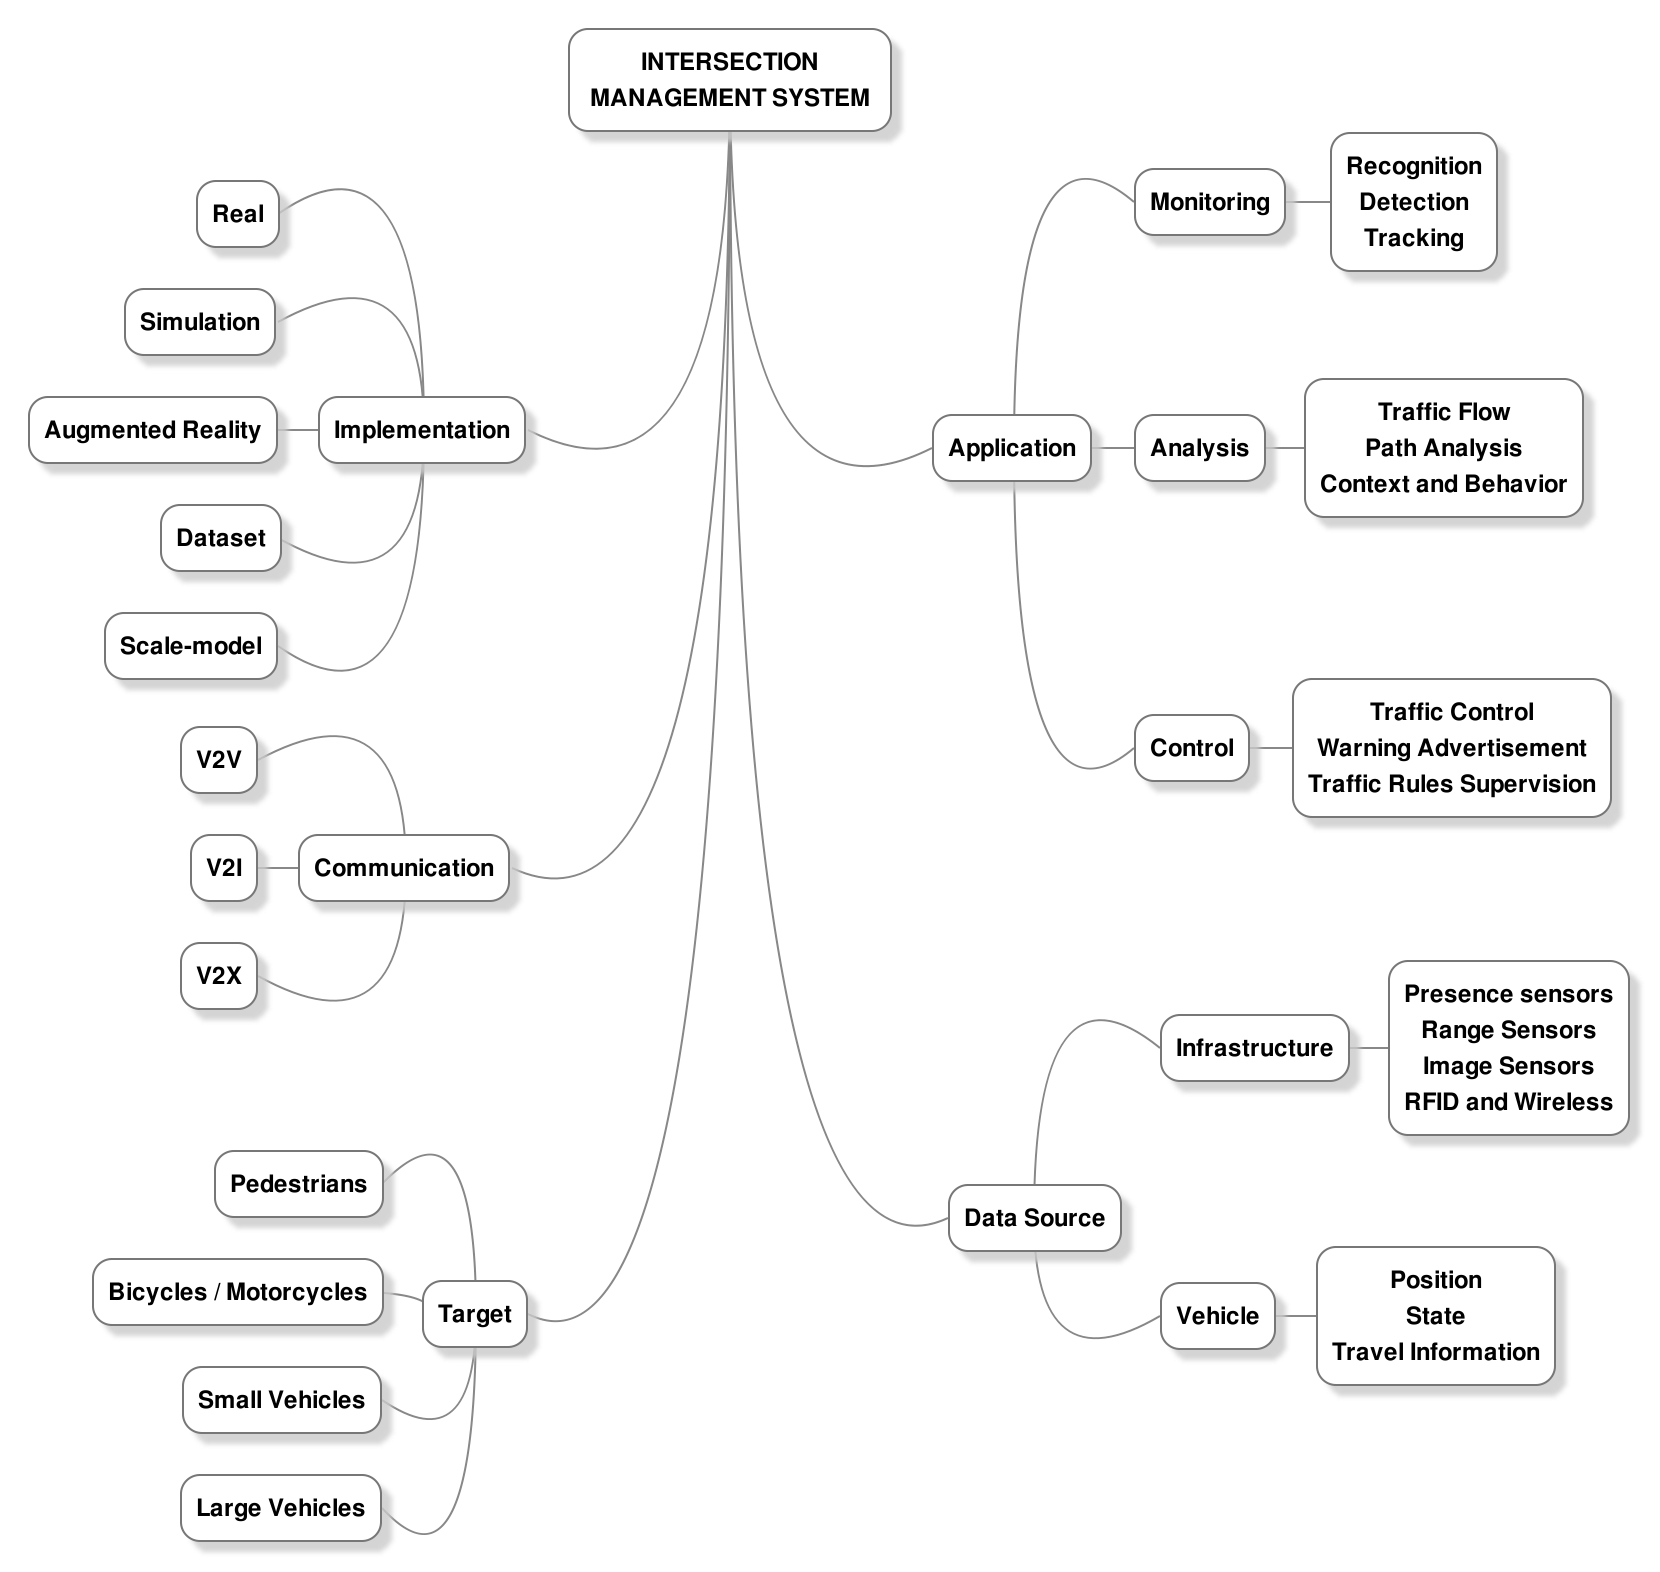
\includegraphics[scale=0.2125]{fig/2/ims_graph2.png}
\caption{Components of an Intersection Management System application.}
\label{imsComps}
\end{figure}

\subsubsection{Application}

Application component could be seen as the final objective of the system. Generally, this includes high-level tasks like monitoring, analysis or control. Monitoring or surveillance systems execute actions like recognition, detection and/or tracking of objects in the scene. 
Other systems analyse the behaviour and interactions between detected objects to recognise path patterns, determine the context of the environment and predict some events of interest. In a higher level there are the control or decisions made based on detection of certain traffic conditions to handle traffic lights, control intersection access, generate warnings to drivers or issue traffic tickets when a rule violation exists.

\subsubsection{Data Source}

The origin of data is considered an independent component because of the variety of possible sources and posterior processing stages. From infrastructure side, data can be captured using a wide range of sensors like inductive loops, lasers, lidars and cameras. Also, monitoring connections to networks, like bluetooth, to estimate vehicle traffic through a place, have been used recently \cite{Friesen2013, Friesen2014}. On the other side, data from vehicles is also useful for the system to enhance its representation of the scene and take decisions. This could be low-level data like vehicle state variables, for example, speed, orientation, acceleration, etc., or high-level data like travel information.


\subsubsection{Target}

In an intersection many objects of different kinds interact between them. Pedestrian and vehicles are found at intersections, and latter includes bicycles, motorcycles, cars, vans, buses, trucks and some other types of vehicles. For this reason some applications are designed for a specific element or group of elements. Pedestrian tracking, motorcycles recognition or car counting are examples of targeted applications.

\subsubsection{Communication}

One of the keypoints of ITS is how information technologies and communication advances are included in transportation. The main goal of this is to allow that information to be shared between vehicles and infrastructure entities. For this reason, 3 communication approaches appear: Vehicle-to-vehicle or Inter-vehicle communication (V2V), vehicle-to-infrastructure communication (V2I) and vehicle to both vehicle and infrastructure (V2X). Several protocols and standars have been proposed for these communication approaches, for example DSRC, WAVE and IEEE 802.11p, but research and development on this component is still active.

\subsubsection{Implementation}

Not all IMS applications are implementable on a real scenario, maybe because is not the scope of the application or because it is in a early stage and it could be validated in other ways. This types of developments are sometimes implemented and evaluated using simulators, making functional prototypes or deploying scale-models. Some other projects use datasets to evaluate new algorithms and data processing techniques, and then compare obtained results with previous works. Augmented reality is also used as a tool for evaluating and validate developmens, taking advantage of the interaction of a real system with a simulated/artificial scenario.

%many approaches have been proposed for information capture stage, both taking data from vehicle or from the infrastructure. For example, monitoring mobile wireless network like Bluetooth \cite{Friesen2013}, detecting vehicle presence using inductive loops or RFID tags, identifying vehicles and pedestrian using cameras \cite{Buch2011, Strigel2013}, single or multiple laser-scanners \cite{Meissner2010, Meissner2012, Zhao2006, Zhao2008, Zhao2012}, and multi-sensor integrated systems \cite{Meissner2013, Meissner2013a, Meissner2014, GoldHammer2012, Zhao2009}.

%Other application are traffic-control oriented, rather than to sensing and data-processing stage. The aim of these applications are to maximise vehicle flow, reduce accidents and improve safety. Many works have been done and although their objective is the same, are diverse between them regarding its communication approach (V2V, V2I or V2X), sensors and information that are used, the execution scenario (simulation, real implementation or augmented reality) and the nature of vehicle driving (Human driver or autonomous vehicles).

%El monitoreo en las intersecciones viales es una tarea requerida en los sistemas inteligentes de transporte para aplicaciones de alto nivel como  an\'{a}lisis de tr\'{a}fico, conteo y  clasificaci\'{o}n de veh\'{i}culos, detecci\'{o}n de eventos, prevenci\'{o}n de accidentes y aplicaciones de seguridad y vigilancia. Para cumplir con estas tareas se han propuesto diversas soluciones para obtener la informaci\'{o}n del entorno, ya sea proveniente de los veh\'{i}culos, por ejemplo monitoreando conexiones a redes m\'{o}viles, como Bluetooth \cite{Friesen2013}, detectando su presencia usando sensores inductivos o etiquetas RFID, y tambi\'{e}n tomando datos desde la infraestructura, usando c\'{a}maras  \cite{Buch2011}, sensores l\'{a}ser o arreglos de estos \cite{Zhao2012} o sistemas que integran m\'{u}ltiples tipos de sensores \cite{Zhao2009}\cite{Pyykonen2010}. Otras aplicaciones adem\'{a}s de monitorear y supervisar las intersecciones, est\'{a}n orientadas al control del tr\'{a}fico en estas con  el objetivo de maximizar el flujo, disminuir la accidentalidad y aumentar la seguridad. Diversos trabajos se han hecho y aunque su finalidad es similar, existe variedad entre s\'{i}, ya sea seg\'{u}n el tipo de comunicaci\'{o}n en la que se basan (V2V, V2I o V2X), el tipo de sensores e informaci\'{o}n que usan, el entorno de ejecuci\'{o}n (simulaci\'{o}n, real o realidad aumentada) y el tipo de veh\'{i}culos (con conductores humanos o veh\'{i}culos aut\'{o}nomos).

%In \cite{Ball2010} and \cite{Azimi2012}, intervehicular-communication based architectures are proposed. In these, each vehicle send to the others its own information about position, velocity, destination and more, and then they coordinate how the access to the intersection should be done. In \cite{Guerrero-Ibanez2013}, is presented a system capable of work in V2I mode, additional to V2V, using inductive loops and RFID information for detecting vehicles. The information is gathered by an intersection controller which manage the access to the crossroad. Another V2I based systems is presented in \cite{Basma2011}, where wireless magnetic nodes are used to detect presence and to send data to a base station, which determines possible collisions and warns driver through a visualisation system in infrastructure. Furthermore, in \cite{Dresner2008} and \cite{CondeBento2012}, are presented simulation-based systems for traffic controlling, using agents and applied to autonomous vehicles. In \cite{Quinlan2010}, an augmented reality implementation of the system proposed in \cite{Dresner2008} is done. In this work, approaching vehicles request to an intersection manager for authorisation to cross and is the manager which decides if it is safe to cross or not, depending on the defined traffic policies.

%En \cite{Ball2010} y \cite{Azimi2012} se proponen arquitecturas basadas en comunicaci\'{o}n intervehicular, donde cada auto env\'{i}a a los dem\'{a}s informaci\'{o}n correspondiente a su posici\'{o}n, velocidad, destino y otros datos, y as\'{i} coordinan el acceso a la intersecci\'{o}n. En \cite{Guerrero-Ibanez2013} se presenta un sistema que adem\'{a}s de trabajar en modo V2V, presenta la opción V2I que incluye sensores inductivos y m\'{o}dulos RFID para detectar veh\'{i}culos. La informaci\'{o}n adquirida es procesada por un controlador de intersecci\'{o}n, el cu\'{a}l se encarga de administrar el ingreso al cruce vial. Otro sistema basado en V2I es \cite{Basma2011} donde tambien se usan nodos de sensores magnéticos inalámbricos que se comunican con una estación base, la cual mediante algoritmos de predicción determina posibles colisiones y advierte a los conductores mediante un sistema de visualización en la infraestructura. Por otro lado, \cite{Dresner2008} y \cite{CondeBento2012} presentan aplicaciones en simulación para el control de las intersecciones usando agentes y aplicado en vehículos autónomos. En \cite{Quinlan2010} se hace una implementación en realidad aumentada del sistema propuesto por Dresner y Stone \cite{Dresner2008}. En esta implementación, los vehículos que se aproximan a la intersección solicitan autorización al controlador para ingresar y es este quien decide cuando pueden cruzar, dependiendo de las politicas de administración definidas.

%\subsection{Taxonomy}

\subsection{Developments in Intersection Management Systems}

\section{Conclusions}

Multisensor data fusion can be defined as the process of combine, merge or integrate data from homogeneous or heterogeneous set of sensors in order to get a better representation of a process, the environment or a situation, through the inference of underlying information and the improve of quality of data. Depending of the nature of the sensors and the source of information, fusion can be done in several manners, i.e., sensor-level fusion, feature-level fusion or decision-level fusion.

Several models, architectures and frameworks have been proposed in literature; some of them to show how a data fusion system should work and some other providing guidelines on how to implement it in a given application. Also, a wide range of algorithms have been used to perform fusion of data, some classified by the nature of the fusion or by the nature of the data, but is finally the environment and the application itself which determines the approach to use.

On the other hand, intersection management systems are highly required to improve safety and mobility in transportation, due to the high complexity present in these places, for drivers and authorities too. There is not an IMS application that address all the needs and problems in an intersection, for this reason many developments with narrow scopes and many topics involved have been proposed through the years. To handle all these works and proposals, a new component-based classification scheme for IMS application has been proposed.
%\end{document}